\documentclass[11pt]{article}
\usepackage[a4paper,margin=21mm]{geometry}
\usepackage[no-math]{fontspec}
\setmainfont{Latin Modern Roman}
\newfontfamily\CJKfont{Noto Serif CJK SC}
\XeTeXlinebreaklocale "zh"
\XeTeXlinebreakskip=0pt plus 1pt
\usepackage{amsmath,amssymb,amsthm,amscd,graphicx,color}
\usepackage{xurl}
\usepackage[unicode,hidelinks]{hyperref}
\allowdisplaybreaks
\setlength\emergencystretch{3em}
\numberwithin{equation}{section}
\numberwithin{equation}{section}

\newtheorem{Theorem}{Theorem}[section]
\newtheorem{Corollary}[Theorem]{Corollary}
\newtheorem{Lemma}[Theorem]{Lemma}
\newtheorem{Proposition}[Theorem]{Proposition}
{ \theoremstyle{definition}
	\newtheorem{Definition}[Theorem]{Definition}
	\newtheorem{Note}[Theorem]{Note}
	\newtheorem{Example}[Theorem]{Example}
	\newtheorem{Remark}[Theorem]{Remark} }

\usepackage[all]{xy}


\def\KK{\ensuremath\mathbb{K}}
\def\MM{\ensuremath\mathbb{M}}
\def\BB{\ensuremath\mathbb{B}}
\def\GL{\ensuremath\mathbf{GL}}
\def\UU{\ensuremath\mathbf{U}}
\def\PP{\ensuremath\mathbb{P}}
\def\CC{\ensuremath{\mathbb{C}}}
\def\NN{\ensuremath{\mathbb{N}}}
\def\QQ{\ensuremath{\mathbb{Q}}}
\def\RR{\ensuremath{\mathbb{R}}}
\def\ZZ{\ensuremath{\mathbb{Z}}}

\newcommand{\profinQ}{\mathfrak{Q}}
\newcommand{\reals}{\mathbb{R}}
\newcommand{\complexs}{\mathbb{C}}
\newcommand{\naturals}{\mathbb{N}}
\newcommand{\integers}{\mathbb{Z}}
\newcommand{\rationals}{\mathbb{Q}}
\newcommand{\quaternions}{\mathbb{H}}
\newcommand{\hyperbolic}{\mathbb{H}}
\newcommand{\K}{\mathbb{K}}
\newcommand{\realsorcomplexs}{\mathbb{K}}
\newcommand{\finitefield}{\mathbb{F}}
\newcommand{\Proj}{\mathbb{P}}
\DeclareMathOperator{\id}{id}
\DeclareMathOperator{\Ind}{Ind}
\newcommand{\boundary}[1]{\partial#1}
\newcommand{\boundedops}{\mathcal{B}}
\newcommand{\bundleover}{\!\!\downarrow\!\!}
\newcommand{\abs}[1]{\left\lvert#1\right\rvert} %absolute value
%\newcommand{\bigabs}[1]{\left\lvert#1\right\rvert} %absolute value
\newcommand{\norm}[1]{\left\lVert#1\right\rVert}
\newcommand{\generate}[1]{\langle#1\rangle}
\newcommand{\tensor}{\otimes}
\newcommand{\into}{\hookrightarrow}
\newcommand{\onto}{\twoheadrightarrow}
\newcommand{\iso}{\cong}
\newcommand{\disjointunion}{\amalg}
\newcommand{\subgroup}{\leq}
\newcommand{\supergroup}{\geq}
\newcommand{\superset}{\supset}
\newcommand{\normalsubgroup}{\lhd}
\newcommand{\semiProd}{\rtimes}
\newcommand{\semiprod}{\semiProd}
\newcommand{\dividesnot}{\nmid}
\newcommand{\divides}{\mid}
\DeclareMathOperator{\Pos}{Pos}
\DeclareMathOperator{\Aut}{Aut}
\DeclareMathOperator{\supp}{supp} %support
\DeclareMathOperator{\clos}{clos} %closure
\DeclareMathOperator{\im}{im} %image
\DeclareMathOperator{\vol}{vol} %Volume
\DeclareMathOperator{\diam}{diam} %Diameter
\DeclareMathOperator{\dist}{dist} %Distance
\DeclareMathOperator{\ord}{ord} %order
\DeclareMathOperator{\End}{End} %Endomorphisms
\DeclareMathOperator{\Hom}{Hom} %Homomorphisms
\DeclareMathOperator{\Span}{span}
\DeclareMathOperator{\spin}{spin}
\DeclareMathOperator{\diag}{diag}
\DeclareMathOperator{\spec}{Spec}
\DeclareMathOperator{\trace}{trace}
\DeclareMathOperator{\tr}{tr}
\DeclareMathOperator{\pr}{pr}
%\DeclareMathOperator{\res}{res} %Restriction
\DeclareMathOperator{\grad}{grad} %Restriction
% \DeclareMathOperator{\Sp}{Sp} %Spur % schon definiert???
\DeclareMathOperator{\fl}{f\/l} %flip
\DeclareMathOperator{\coker}{coker}
\DeclareMathOperator{\Char}{Char}
\DeclareMathOperator{\ind}{ind}
\DeclareMathOperator{\sgn}{sgn}
\DeclareMathOperator{\Ric}{Ric} % Ricci curvature
\DeclareMathOperator{\scal}{scal} % Scalar curvature
\DeclareMathOperator*{\dirlim}{dirlim}
\DeclareMathOperator*{\invlim}{invlim}
\DeclareMathOperator{\rank}{rank}
\DeclareMathOperator{\coind}{coind}
\DeclareMathOperator{\res}{res}
\newcommand{\bigdisjointunion}{\bigsqcup}
\DeclareMathOperator{\Orb}{Orb}
\DeclareMathOperator{\GTOP}{G-TOP}
\newcommand{\forget}[1]{}
\newenvironment{Forget}{}{}
\newcommand{\innerprod}[1]{\langle #1 \rangle}

\begin{document}
\begin{center}\Large Equivariant Stolz R-group invariance under a 2-connected G-map in dimensions at least six\end{center}
\noindent\textbf{Stable ID:} 809\quad\textbf{Author:} Massimiliano Puglisi; Thomas Schick; Vito Felice Zenobi\par
\noindent\textbf{Work:} Stolz Positive Scalar Curvature Structure Groups, Proper Actions and Equivariant 2-Types\par
\noindent\textbf{Source:} \url{https://sigma-journal.com/2025/093/}\par
\noindent\textbf{Version:} Official SIGMA 21 (2025) journal PDF and native TeX; acquired 2026-09-30; exact bytes pinned by SHA256\par
\noindent\textbf{Rights:} CC BY 4.0. Authors retain copyright. \url{https://creativecommons.org/licenses/by/4.0/}. Reuse and typesetting adaptation; original language and mathematical content preserved.\par
\noindent\textbf{Difficulty (prior selection preserved):} {\CJKfont H2: Surjectivity and injectivity require arranging equivariant Morse handles on bordisms with corners, separating low-dimensional extension obstructions from codimension-at-least-three metric surgery, and preserving vertical boundary data. The relative factorization and surgery constructions are retained; a formal homotopy-invariance assertion would omit the core.}\par
\medskip\noindent\textbf{Editorial boundary note (not author text):} Complete original Theorem4.1, including both surgery-based surjectivity and relative lifting/injectivity arguments. All hypotheses and conventions for discrete proper G-actions, fixed-pointwise G-connectivity, G-CW-complexes, Spin bordism, positive-scalar-curvature R-cycles and their bordisms are retained, with the complete human-authored equivariant Stolz exact-sequence core. The three original bordism/corner illustrations and native XY equivariant-map diagram are retained; all proof mathematics and text are editable. Later universal-space/fundamental-groupoid construction and consequences are excluded. Standard equivariant cellular/Whitehead lifting, equivariant Morse handles and Gromov–Lawson surgery are retained as exact author prerequisites with original theorem locators, not recursively reproved. Source CRLF lines are normalized to LF in excerpts only; original bytes stay separately hash-bound. No variable/name/formula repair or mathematical refereeing is performed.\par
\medskip\hrule\medskip\noindent\textbf{Author text begins below.}\par
\setcounter{section}{1}
% Original source lines 234--731
\section{Proper actions of discrete groups}

Let us fix throughout a discrete group $G$.

\begin{Definition}
	A $G$-CW-complex X is a $G$-space together
	with a $G$-invariant filtration
	\[
\varnothing = X^{(-1)}\subseteq X^{(0)} \subseteq X^{(1)} \subseteq \dots \subseteq X^{(n)}\subseteq \dots \subseteq\bigcup_{n\geq0}X^{(n)}=X
\]
	such that $X$ carries the colimit topology with respect to this filtration and for each $n\geq0$
	the space $X^{(n)}$ is obtained from $X^{(n-1)}$ by attaching equivariant $n$-dimensional
	cells, i.e., there exists a $G$-pushout
	\[
	\xymatrix{\displaystyle\bigsqcup_{i\in I_n}G/H_i\times S^{n-1}\ar[r]\ar[d]& X^{(n-1)}\ar[d]\\
		\displaystyle\bigsqcup_{i\in I_n}G/H_i\times D^n\ar[r]& X^{(n)}.}
	\]
	
	Note that the $G$-CW-complex $X$ defines its \emph{isotropy family}
	$\mathcal{I}(X)$ of subgroups of $G$ where~$H$ belongs to $\mathcal{I}(X)$ if and
	only if the fixed point set $X^H$ is non-empty or in other words if and only
	if $X$ contains a $G$-cell $G/K\times D^n$ where a conjugate of $H$ is
	contained in $K$.
\end{Definition}

We recall the concept of a family of subgroups which we just have used.

\begin{Definition}
	Let $G$ be a discrete group. A \emph{family of subgroups $\mathcal{F}$} is a
	set of subgroup of $G$ which is closed under conjugation and is closed under passing
	to smaller subgroups.
	
	Significant examples of such families of subgroups are $\mathcal{FIN}$, the family of all finite subgroups, or
	$\mathcal{ALL}$, the family of all subgroups.
\end{Definition}


Let us fix some notation.
\begin{Definition}
	Let $f\colon X \rightarrow Y$ be a continuous $G$-equivariant map between
	$G$-spaces. We will denote by $f^H\colon X^H\to Y^H$ the restriction of $f$
	to the $H$-fixed point sets, with $H$ a subgroup of~$G$.
\end{Definition}

\begin{Definition}
	We say that $f$ is cellular if $X$ and $Y$ are $G$-CW-complexes and, denoting by~$X^{(k)}$ the \textit{k-skeleton} of X, one has $f\bigl(X^{(k)}\bigr) \subseteq Y^{(k)}$.
\end{Definition}
The well-known and important cellular approximation theorem extends to the equivariant context (compare \cite[Theorem~2.1]{ttd}).

\begin{Theorem} \label{cellular}
	Let $f\colon X\to Y$ be a $G$-map. Then there exists a G-homotopy $h\colon X\times I\to Y$ such that $h_0:= h_{X\times\{0\}}=f$ and $h_1:= h_{X\times\{1\}}$ is cellular.
\end{Theorem}

We also have an equivariant version of the Whitehead Theorem for $G$-CW-complexes.

\begin{Definition}\label{def:connectedness}
	Consider a function $\nu\colon \mathcal{ALL}\to\mathbb{N}$. Then we say that
	$f$ is~$\nu$-connected if~$f^H$ is~$\nu(H)$-connected for all $H\in
	\mathcal{F}$, namely the induced maps are isomorphisms on the first
	$\nu(H)-1$ homotopy groups of (all components of) $X^H$ and $Y^H$ and a
	surjection on the $\nu(H)$-th one.
	In particular, we say that it is {$k$-connected} if $\nu$ is constantly equal to $k$.
	
	Moreover, we say that a relative $G$-CW-complex $(X,A)$ has dimension less or equal to $\nu$ if the cells in $X\setminus A$ are of the form $G/H\times D^k$ with $k\leq\nu(H)$.
\end{Definition}
\begin{Proposition}[{compare \cite[Proposition~2.6]{ttd}}] \label{whitehead}
	Let $f\colon B\to C$ be a $\nu$-connected map between $G$-CW-complexes and $A$
	another
	$G$-CW-complex. Write $[A,B]^G$ for the set of $G$-homotopy classes of
	$G$-maps from $A$ to $B$. Then
	\begin{equation*}
		f_*\colon\ [A,B]^G\to [A,C]^G
	\end{equation*}
	is surjective $($or
	bijective, respectively$)$ if $\dim A\leq\nu$ $($or $\dim A<\nu$, respectively$)$.
\end{Proposition}

Note that the classical Whitehead theorem is a consequence, using $A=C$
and $A=B$ and identity maps.

\section{The Stolz exact sequence}
	
\begin{Definition}\label{def:Stolz_groups}
		Let $X$ be a $G$-CW-complex. We then define the following groups:		
		\begin{itemize}\itemsep=0pt
			\item $\Omega^{\rm spin}_{n}(X)^{G}$ is the $G$-equivariant \textit{spin
				bordism} group: a cycle here is given by a pair $(M,f)$, where $M$ is an
			$n$-dimensional spin-manifold with cocompact spin-structure
			preserving\footnote{That is, with a lift of the action to the Spin principal
				bundle.} action of $G$ and with a $G$-equivariant
			reference map $f\colon M\to X$. Two cycles $(M,f)$ and~$\bigl(M',f'\bigr)$ are
			equivalent if there is a cocompact spin $G$-bordism $W$ from $M$ to $M'$
			and there exists a $G$-equivariant reference map $F\colon W\to X$
			extending $f$ and $f'$.
			\item $\mathrm{Pos}^{\rm spin}_{n}(X)^{G}$ consists of cycles $(M,f,g)$, where the pair
			$(M,f)$ is as before and $g$ is a~$G$-invariant metric with positive
			scalar curvature on $M$. Two such cycles $(M,f,g)$ and~$\bigl(M',f',g'\bigr)$ are
			equivalent if there exists a~spin bordism $(W,F)$ as before, along with a~$G$-invariant metric $g_W$ on $W$ which is of product type near the
			boundary which restricts to $g$ on $M$ and to $g'$ on $M'$.
			\item $R^{\rm spin}_{n}(X)^{G}$ is the bordism group of spin $G$-manifolds with
			boundary (possibly empty) of dimension $n$, together with a $G$-invariant
			Riemannian metric of positive scalar curvature on the boundary. Bordisms are then manifolds with
			corners. In particular, $(M,f,g)$ and $\bigl(M',f',g'\bigr)$ are equivalent if there
			exists a $G$-bordism $(W,F,\bar{g})$, where $W$ is a bordism between $M$
			and $M'$ and the resulting bordism $\partial_0 W$ between $\partial M$ and
			$\partial M'$ carries a $G$-invariant
			metric $\bar{g}$ with positive scalar curvature, so that it is a
			bordism between~${\bigl(\partial M,\partial f,g\bigr)}$ and
			$\bigl(\partial M',\partial f',g'\bigr)$ in the sense of $\mathrm{Pos}^{\rm spin}_{n-1}(X)^{G}$.
		\end{itemize}
		
		Each of these sets is equipped with an abelian group structure given by
		disjoint union of manifolds and is covariantly functorial in $X$ as follows: a $G$-equivariant map of $G$-CW-Complexes~${\varphi\colon X \rightarrow Y}$ induces a mapping $\varphi_{*}$ on these groups
		by post-composing the reference maps with~$\varphi$.
	\end{Definition}
	
	\begin{Remark}
		Note that for each cycle $f\colon M\to X$ in $\Omega_n^{\rm spin}(X)^G$ the
		isotropy of $M$ is restricted to belong to the family $\mathcal{I}(X)$
		(because the image under the equivariant map $f$ of a point $x\in M$ fixed by a subgroup $H$ of
		$G$ must also be fixed by $H$, and is a point in $X$).
		
		If we want to restrict the isotropy even further, to live in a family
		$\mathcal{F}$ of subgroups of $G$, we can replace the space $X$ by $X\times
		E_{\mathcal{F}}G$ where $E_{\mathcal{F}}G$ is the universal $G$-CW-complex
		with isotropy family $\mathcal{F}$. This space is characterized by the property
		that $E_{\mathcal{F}}G^H$ is empty if $H\notin \mathcal{F}$ and~$E_{\mathcal{F}}G^H$ is contractible if $H\in\mathcal{F}$, in particular $\mathcal{I}(E_{\mathcal{F}}G)=\mathcal{F}$. It exists for
		each family $\mathcal{F}$ and it is unique up to $G$-equivariant homotopy
		equivalence. It has the universal property that a~$G$-CW-complex~$X$ with
		isotropy contained in $\mathcal{F}$ has a unique homotopy class of $G$-maps
		to~$E_{\mathcal{F}}G$. These spaces were introduced and studied in \cite{tomDieck,ttd}.
	\end{Remark}

\begin{Proposition}\label{prop:Stolz_seq}
		The abelian groups defined in Definition~{\rm\ref{def:Stolz_groups}} fit into the
		following $G$-equivari\-ant version of the Stolz positive scalar curvature exact sequence:
		\[
			\cdots \to R^{\rm spin}_{n+1}(X)^{G} \to \mathrm{Pos}^{\rm spin}_{n}(X)^{G} \to \Omega^{\rm spin}_{n}(X)^{G} \to R^{\rm spin}_{n}(X)^{G} \to \cdots,
		\]
		where the first map sends a manifold to its boundary, the second one
		is the forgetful map $($i.e., it forgets the metric of positive scalar curvature$)$
		and the last one considers a closed manifold as a~manifold with empty boundary.
	\end{Proposition}
	\begin{proof}
		This is a rather direct consequence of the definitions and well known to the
		experts, at least non-equivariantly, stated, e.g., in \cite[long exact sequence~(4.4)]{Stolz} (but
		without proof). The
		argument for the
		$G$-equivariant case is exactly the same as the classical non-equivariant
		situation. As we are not aware of a treatment available in the journal
		literature, we follow the referee's suggestion and give a complete account
		of the argument here.
		
		First, that the composition of two consecutive maps is zero indeed is a
		direct consequence of the definitions:
		\begin{itemize}\itemsep=0pt
			\item Given $[W,f,g]\in R^{\rm spin}_{n+1}(X)^G$, its image in $\Omega_n(X)^G$ is
			represented by $(\boundary W,f|_{\boundary W})$ which indeed is a boundary, hence represents
			$0$.
			\item Given $[M,f,g]\in \mathrm{Pos}_n^{\rm spin}(X)^G$, its image in $R^{\rm spin}_n(X)^G$ is
			the manifold $M$ with empty boundary. It is bordant in $R^{\rm spin}_n(X)^G$
			to $\varnothing$ and hence represents $0$ via the
			bordism $M\times [0,1]$, where $(M\times \{1\},g)$ is a positive scalar curvature bordism of
			$\varnothing =\boundary M$ to $\varnothing=\boundary\varnothing$.
			\item Given $[M,f]\in \Omega^{\rm spin}_n(X)^G$, its image in
			$\mathrm{Pos}_{n-1}^{\rm spin}(X)^G$ is represented by $\boundary M=\varnothing$, hence
			represents $0$.
		\end{itemize}
		
		For the opposite inclusions of the kernels in the image, the constructions
		are almost as straight-forward:
		\begin{itemize}\itemsep=0pt
			\item Assume that $[M,f]\in \Omega^{\rm spin}_n(X)^G$ is mapped to $0$ in
			$R^{\rm spin}_n(X)^G$. This means that there is a null-bordism $(W,F)$. In the
			case at hand, $\boundary W$ has two disjoint parts: on the one hand~$(M,f)$
			and on the other hand $\bigl(M',f',g'\bigr)$ which is a bordism from $\boundary
			M=\varnothing$ to $\boundary\varnothing=\varnothing$ and which is equipped with
			a metric $g$ of positive scalar curvature. But this means, by definition,
			that $[M,f]=\big[M',f'\big]\in \Omega^{\rm spin}_n(X)^G$ where $M'$ is equipped with a
			metric $g$ of positive scalar curvature. Hence we have the preimage
			\smash{$\big[M',f',g\big]\in \mathrm{Pos}^{\rm spin}_n(X)^G$} of the initial equivariant bordism class
			$(M,f)$.
			\item Assume that $[M,f,g]\in \mathrm{Pos}^{\rm spin}_n(X)^G$ is mapped to $0$ in
			$\Omega^{\rm spin}_n(X)^G$. This means that there is a bordism $(W,F)$ with
			$\boundary(W,F)=(M,f)$. But then $[W,F,g]$ represents a class in~$R^{\rm spin}_{n+1}(X)^G$ which is mapped to $[M,f,g]\in \mathrm{Pos}^{\rm spin}_n(X)^G$.
			\item Finally, assume that \smash{$[W,f,g]\in R^{\rm spin}_{n+1}(X)^G$} is mapped to $0$
			in $\mathrm{Pos}_n^{\rm spin}(X)^G$. This means that there is a second bordism
			$\bigl(W',f',g'\bigr)$ whose boundary is $(\boundary W,f|_{\boundary W},g)$.
			We now consider the closed $G$-manifold $Z:= W\cup_{\boundary W} W'$ with
			map $F:= f\cup_{\boundary W} f'\colon Z\to X$ and the bordism $B:=Z\times
			[0,1]$ with map $F\circ \operatorname{pr}_Z\colon B\to X$. The boundary of $B$ consists
			of three parts: the internal boundary $W'$ between $\boundary W$ and
			$\varnothing =\boundary Z$, equipped with the metric~$g'$ of positive scalar
			curvature extending $g$. The other two boundary parts are $W$ and $Z$, and
			by definition $(B,F\circ \operatorname{pr}_Z, g')$ is a bordism in $R^{\rm spin}_n(X)^G$
			between $(W,f,g)$ and $(Z,f,\varnothing)$ and~${[Z,f]\in
			\Omega^{\rm spin}_n(X)^G}$ represents a preimage of $[W,f,g]\in R^{\rm spin}_n(X)^G$.\hfill $\qed$
		\end{itemize} \renewcommand{\qed}{}
	\end{proof}
	
Let $X$ be a connected $G$-CW-complex with $x_0\in X$ and fundamental group
	$\pi_1(X,x_0)$. Let
	\begin{equation*}
		\pi\colon\ \bigl(\tilde{X},\tilde x_0\bigr)\to (X,x_0)
	\end{equation*}
	be the
	associated universal covering projection. Then the
	proper $G$-action on $X$ lifts to a $\widetilde{G}$-action on $\tilde{X}$,
	where
	\begin{equation*}
		1\to\pi_1(X,x_0)\to \widetilde{G}\to G\to 1
	\end{equation*}
	is an extension of
	discrete groups
	defined as follows: the elements of $\widetilde{G}$ are pairs
	$\bigl(\alpha\colon\tilde X\to\tilde X,g\bigr)$ where $g\in G$ and $\alpha$ covers the
	action map of $g$ on $X$. We define the multiplication by composition of the
	maps $\alpha$ and
	multiplication in $G$.
	
	Note that, by covering theory, because $\tilde X$
	has trivial fundamental group, indeed for each $\tilde x_1\in\tilde X$ with
	$\pi(\tilde x_1)=g\cdot \pi(\tilde x_0)$
	there is a unique lift of the action map sending $\tilde x_0$ to $\tilde
	x_1$.
	
	The projection map $\widetilde{G}\to G$ sends $(\alpha,g)$ to $g$. By
	the above consideration, this map is surjective and its kernel consists of
	the deck transformations which, by covering theory, are identified with
	$\pi_1(X,x_0)$.
	
	\begin{Remark}
		The Stolz exact sequence of Proposition~\ref{prop:Stolz_seq} can always be
		reduced to a sequence where the space $X$ is connected. This is done in two
		steps:
		\begin{enumerate}\itemsep=0pt
			\item[(1)] For every component $X_c$ of $X$ consider the induced $G$-invariant
			subspace $G\cdot X_c$. We then have a disjoint union decomposition into
			$G$-invariant subsets $X=\bigdisjointunion G\cdot X_c$ with~$X_c$ connected
			(choosing one representative in each $G$-orbit of components).
			Clearly, every group in the Stolz exact sequence and the whole sequence
			then split canonically as a~direct product, with one factor for each
			$G\cdot X_c$.
			\item[(2)] For a $G$-space $Y=G\cdot X_c$ with $X_c$ connected, consider the
			subgroup $G_0\subset G$ of all elements which map $X_c$ to itself. Then
			$X_c$ is a $G_0$-space and $Y$ is obtained by ``induction'': $Y=
			G\times_{G_0}X_c$. Whenever we have a $G$-map $f\colon M\to Y$ which
			could be part of a~cycle or a bordism for the groups in the Stolz exact
			sequence, then we obtain~${M_0:=f^{-1}(X_c)}$ a union of components of $M$
			on which $G_0$ acts (restricting the action of $G$ on $M$). Then~${f|_{M_0}\colon M_0\to X_c}$ is a $G_0$-equivariant map and we obtain $M$ and
			$f$ by induction: $M=G\times_{G_0} M_0$ and $f=\id_G\times_{G_0}
			f|_{M_0}$.
			It follows that induction gives an isomorphism (already on the level of
			cycles and relations)
			\begin{equation*}
				\mathrm{ind}_{G_0}^G\colon\ R^{\rm spin}_*(X_c)^{G_0}\to R^{\rm spin}_*(Y)^G
			\end{equation*}
			and the same for the other groups in the sequence of Proposition~\ref{prop:Stolz_seq}
			and the maps between them.
		\end{enumerate}
	\end{Remark}
	
	\begin{Remark}
		The isotropy family $\mathcal{I}\bigl(\tilde{X}\bigr)$ of the action of $\widetilde{G}$
		on $\tilde{X}$ is precisely the inverse image of $\mathcal{I}(X)$ under the projection
		\smash{$\widetilde{G}\to G$}.
		
		This again follows from covering theory: if we fix $x\in X$ with lift
		$\tilde x\in\tilde{X}$ and a subgroup $H$ of~$G$ fixing $x$ we have a
		canonical split $H\to \widetilde{G}$ sending $h\in H$ to the unique pair
		$\bigl(\alpha\colon \tilde X\to \tilde{X},h\bigr)$ such that $\alpha(\tilde x)=\tilde
		x$.
	\end{Remark}
	
	
	Then we have the following easy identification.
	\begin{Proposition}\label{extension}
		The $G$-equivariant Stolz exact sequence associated to $X$ is isomorphic to
		the $\widetilde{G}$-equivariant Stolz exact sequence associated to
		$\tilde{X}$.
	\end{Proposition}
	\begin{proof}
		The action of $\pi_1(X)\subset \widetilde{G}$ on $\tilde X$ is
		free. Consequently, for every $\widetilde{G}$-map ${f\colon \bar M\to\tilde X}$ the
		action of $\pi_1(X)$ on $\bar M$ is free. We can therefore quotient out this
		action and obtain a~cycle~${M:=\bar M/\pi_1(X)\to X}$ with residual action of
		$G:=\widetilde{G}/\pi_1(X)$.
		Vice versa, given a~$G$-map~${f\colon M\to X}$ we can pull back $\tilde X\to
		X$ along $f$ and obtain a $\pi_1(X)$-covering $\tilde M\to M$ with map
		$\tilde f\colon \tilde M\to \tilde X$. Because $f$ is a $G$-map, it is
		straightforward to pull back
		also the action of $\widetilde{G}$ to an action on $\tilde M$ which covers
		the action of $G$ on $M$ and such that $\tilde f$ is a $\widetilde{G}$-map
		(indeed, the $\widetilde{G}$-action on $\tilde M$ is defined mapping a point
		$(m,\tilde x)\in \tilde M\subset M\times \tilde X$ by
		$(\alpha,g)\in\widetilde{G}$ to $(gm,\alpha(\tilde x))$).
		
		The same construction gives a bijection between $G$-invariant metrics on $M$
		and $\widetilde{G}$-invariant metrics on $\tilde M$, and also works for
		bordisms.
		These constructions are clearly inverse to each other and preserve all
		additional structure and define the required bijections.
	\end{proof}
	
	\begin{Remark}
		For the paper at hand, the transition to the universal covering as in
		Proposition~\ref{extension} is not really relevant. However, in other
		situations this point of view is really fruitful. To our knowledge,
		essentially all information about non-triviality of the groups
		$R^{\rm spin}_n(X)$ and~$\mathrm{Pos}_n^{\rm spin}(X)$ use higher index theory of the Dirac
		operator. A particularly transparent way to do this is to use the
		equivariant Dirac operator on the universal covering. This essentially means
		that one applies the isomorphism between the groups ``downstairs'' for $X$ and the
		$\pi_1(X)$-equivariant groups ``upstairs'' for the universal covering
		$\tilde X$, as we have already mentioned in the introduction.
		
		It
		is pretty obvious that the same observation does hold for non-free actions: even
		if we want to understand symmetric metrics of positive scalar curvature on a
		compact manifold $M$ with smooth action of a finite group $\Gamma$, it will
		be very useful to pass to the covering space which also sees the symmetries
		induced by the non-trivial fundamental group. This strategy has already been
		implemented in \cite[Section 5]{XieYu}
		and \cite{XieYuZeidler}. The first paper constructs the map from the
		equivariant
		Stolz sequence to analysis (in form of the Higson--Roe exact sequence for the
		K-theory of the Roe $C^*$-algebra) in the
		sense of \cite{PiazzaSchick}. The second paper then uses this to explicitly
		distinguish many bordism classes of equivariant positive scalar curvature
		metrics.
	\end{Remark}
	
	
	\subsection{Refinements beyond bordism of positive scalar curvature metrics}
	
	The Stolz positive scalar curvature exact sequence of Proposition
	\ref{prop:Stolz_seq} gives important information about the existence and
	classification of metrics of positive scalar curvature. However, by the very
	definition this information is about \emph{bordism} classes and we are of
	course also interested in a fixed given manifold $M$.
	
	Non-equivariantly, the situation here is very satisfactory: for a given
	connected closed spin manifold $M$ with $\dim(M)\ge 5$, if we use $X=B\pi_1M$
	then $M$ itself admits a metric with positive scalar curvature if (and only
	if) the image of $[u\colon M\to B\pi_1(M)]$ in $R_n^{\rm spin}(B\pi_1(M))$
	vanishes. Moreover, in this case $R_{n+1}^{\rm spin}(B\pi_1(M))$ acts freely and
	transitively on the concordance classes of metrics of positive scalar
	curvature on $M$.
	
	Of course, it would be very desirable to extend such results to the
	equivariant case. Unfortunately, the proof in the non-equivariant case uses as
	an important tool ``handle cancellation'' for Morse functions. It is known
	that equivariantly such cancellation is not even true. Therefore, a~general
	treatment of the equivariant case seems not in reach at the moment. Under very
	special conditions on the action, positive existence results can be
	obtained. The strongest results in this direction we are aware of are obtained
	in \cite{Hanke}. There, also the difficulties are discussed when one attempts
	to obtain more general results. In the paper at hand, we focus on the bordism
	context and do not attempt to contribute to obstruction and classification
	results for G-invariant metrics of positive scalar curvature on a fixed
	manifold $M$.
	
\section[Invariance of R-groups under 2-equivalence]{Invariance of $\boldsymbol{R}$-groups under 2-equivalence}
	
	\begin{Theorem}\label{G2conn}
		Let $f\colon X \rightarrow Y$ be a continuous, $2$-connected $G$-map
		between $G$-CW-complexes $($in particular, it induces a bijection
		between components of fixed point sets and an isomorphism of the
		fundamental groups of all
		components of fixed point sets of $X$ and the corresponding ones of
		$Y)$. Then for $*\ge 6$ the
		functorially induced map
$f_{*}\colon R_{n}^{\rm spin}(X)^{G} \rightarrow R_{n}^{\rm spin}(Y)^{G}
$
		is an isomorphism.
	\end{Theorem}
	\begin{proof}
\!{\it Surjectivity.}\! We start by showing the surjectivity of the map
$f_{*}\colon R_{n}^{\rm spin}(X)^{G} \!\rightarrow\! R_{n}^{\rm spin}(Y)^{G}$.
		Let us consider a class $[W,\varphi\colon W \rightarrow Y, g] \in
		R_{n}^{\rm spin}(Y)^{G}$. We want to find a \textit{bordant} cycle whose reference map factors through $f$.
		
Consider W as a bordism between its boundary $\partial W$ and the empty set
		and choose a~$G$-invariant Morse function $\alpha\colon W\to \RR$ on it with
		critical points rearranged as described in~\cite[Theorem 4.8]{Milnor}, namely
		for any critical points $p_{i}$ and $p_{j}$ such that $f(p_{i}) < f(p_{j})$,
		we have that~${\operatorname{Ind}_f(p_{i}) < \operatorname{Ind}_f(p_{j})}$, where $\operatorname{Ind}_f(p)$ denotes the Morse index at $p$ of the function $f$. Notice that we are going to use the
		enhanced version of this result to the equivariant setting, see for instance
		\cite{Mayer} or \cite{Wasserman}.
		
		Then there exists a suitable $t\in \RR$ such that the subset $W_1:=\alpha^{-1}([0,t])\subset W$ consists only of $G$-handles of dimensions 0, 1 and 2. We immediately obtain a decomposition of $W$ as~${W_{1} \cup W_{2}}$ such that $W_{1}$ is a bordism from the empty set to $M_{1}:=\alpha^{-1}(t)$ and $W_{2}$ a bordism from $M_{1}$ to~$\partial W$.
		Of course, $W_{2}$ has only critical points $p_{i}$ with~$\operatorname{Ind}_{\alpha}(p_{i}) \geq 3$. Consider now the function~$-\alpha$: this is a Morse function on $W_{2}$ seen as a bordism from $\partial W$ to $M_{1}$ with same critical points~$p_{i}$ but with indices now given by $\operatorname{Ind}_{-\alpha}(p_{i})=\dim(W)-\operatorname{Ind}_{\alpha}(p_{i})$. These critical points $p_{i}$ are then associated to $G$-equivariant~${(\operatorname{Ind}_{-\alpha}(p_{i})-1)}$-surgeries, hence of codimension~${\operatorname{Index}_{\alpha}(p_{i})+1}$ which is $\geq 3$.
		
		\begin{figure}[h]
			\centering
			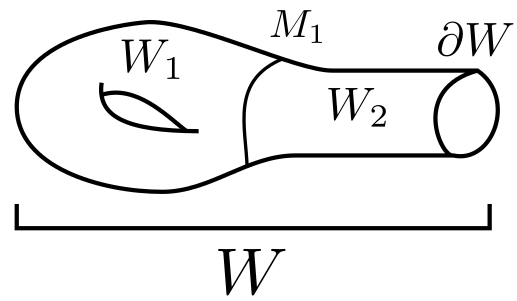
\includegraphics[width=45mm]{W}
		\end{figure}
		
		This allows us to apply the Gromov--Lawson theorem in its $G$-equivariant
		version as it is proved in \cite[Theorem 2]{Hanke}. This implies that we can
		extend the metric with positive scalar curvature $g$ on $\partial W$ to a
		$G$-invariant metric with positive scalar curvature $\bar{g}$ on $W_2$. Let us
		denote by $g_{1}$ its restriction to $M_{1}$.
		Observe that the triad $(W_{1},\varphi_{|W_{1}},g_{1})$ defines a class in~\smash{$R_{n}^{\rm spin}(Y)^{G}$} and the manifold $W \times [0,1]$ provides a bordism between \smash{$(W_{1},\varphi_{|W_{1}},g_{1})$} and $(W,\varphi, g)$.
		
		Consider now the natural $G$-equivariant inclusion of the 2-skeleton given by $i\colon
		Y^{(2)}\hookrightarrow Y$. Here we have the following facts:
		\begin{itemize}\itemsep=0pt
			\item 	Since the manifold $W_{1}$ is obtained from the empty set by attaching $G$-handles of dimension~0,~1 and 2, it is homotopy equivalent to a 2-dimensional $G$-CW-complex. It follows from Theorem~\ref{cellular} that the map $\varphi_1:=\varphi_{|W_{1}}$ factors through $i$ up to homotopy.
			\item Since $f$ is 2-connected, up to $G$-homotopy we can assume that its
			restriction to the 2-skeleton
		\smash{$
				f^{(2)}\colon\ X^{(2)} \rightarrow
				Y^{(2)}\rightarrow Y
			$}
			has a right inverse, i.e., there exists a $G$-equivariant map~${h\colon
			Y^{(2)} \rightarrow X^{(2)}}$ such that $f^{(2)}\circ h$ is homotopic to
			$i$. To see this, observe that the existence of such a map $h$ is guaranteed,
			up to $G$-homotopy, by Proposition~\ref{whitehead}. In fact, since $f^{(2)}$
			is $2$-connected and $Y^{(2)}$ has dimension $\leq 2$, it suffices to apply
			Proposition~\ref{whitehead} with $A=Y^{(2)}$, $B=X^{(2)}$, $C=Y$ and $f=f^{(2)}$ to the
			map $i \in [A,C]^G$. The surjectivity of~$f_*$ then implies the existence
			of $h$.
		\end{itemize}
		Thus, we obtain the following commutative diagram of $G$-equivariant maps
$$%\label{diagram1}
			\xymatrix{W_1 \ar[rr]^{\varphi_1} \ar[d]_{\varphi_1}&& Y & \\
				Y^{(2)} \ar[d]_h \ar[urr]^i & & \\
				X^{(2)} \ar[uurr]_{f^{(2)}} \ar[rr]_j && X\ar[uu]_f}
$$
		and, if we set $\psi:= j\circ h\circ \varphi_1\colon W_1\to X$, we obtain by
		construction that
		\[
f_*[W_1,\psi\colon W_1\to X, g_1]=[W,\varphi\colon W\to Y,g]\in R^{\rm spin}_n(Y)^{G},
\]
 which proves that $f_*$ is surjective.
		
\textit{Injectivity.} In order to prove the injectivity of $f_*\colon R_{n}^{\rm spin}(X)^{G}\to R_{n}^{\rm spin}(Y)^{G} $, let us consider a~class $[W,\varphi\colon W \rightarrow X,g]\in R_{n}^{\rm spin}(X)^{G}$ such that its image $f_{*}[W,\varphi\colon W \rightarrow X,g]$ is equal to the trivial element in $R_{n}^{\rm spin}(Y)^{G}$. This means that there exists
		\begin{itemize}\itemsep=0pt
			\item an $(n+1)$-dimensional $G$-manifold with corners $B$, whose codimension 1
			faces are $W$ itself together with a bordism $V$ from $\partial W$ to the empty set, which intersect in the only codimension 2 face $\partial W=W\cap V$;
			\item a $G$-invariant metric $g_V$ on $V$ of positive scalar curvature of
			product type near the boundary which restricts to the metric $g$ on $\partial
			W$;
			\item a $G$-equivariant map $\Psi\colon B\to Y$ which restricts to
			$f\circ\varphi$ on $W$.

		\end{itemize}
		
		\begin{figure}[h]%\label{B}
\vspace*{-6mm}
			\centering
			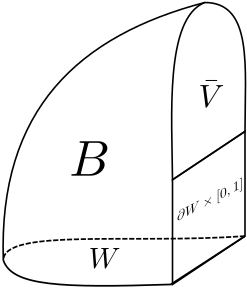
\includegraphics[width=28mm]{B}
		\end{figure}
		
		Consider now a $G$-invariant collar neighborhood of $\partial W$ inside $V$ such that the boundary of $B$ is made of three faces of codimension 1: $W$ on the bottom, $\partial W \times [0,1]$ vertically and~${\bar{V}=V\setminus\partial W \times [0,1)}$ on the top.
		
We want to split the bordism $B$, as we did in the proof of surjectivity, into the composition of two bordisms, first from $W$ to a manifold with boundary $W_1$ and then from $W_1$ to $\bar{V}$, such that the first one involves only handle attachments of dimension less or equal than 2 and the second one only of dimension greater or equal than 3.
		Since the vertical boundary face $\partial W \times [0,1]$ is a cylinder, $B$ can be obtained from $W$ by attaching all the handles to the interior of $W$, away from $\partial W \times [0,1]$.
		Hence we can find a Morse function on $B$ which has all critical points there.

		
Thus, we can decompose $B$ as desired: $B_{1}$ from $W$ to $W_{1}$
		involving only 0, 1, 2 handle attachments and $B_{2}$ from $W_{1}$ to
		$\bar{V}$. We can assume that these two bordisms have vertical
		boundaries faces equal to $\partial W \times [0,1/2]$ and $\partial W
		\times [1/2,1]$, respectively, and therefore that $W_{1}$ has
		boundary equal to $\partial W$.
		
		\begin{figure}[h]%\label{B1-B2}
			\centering
			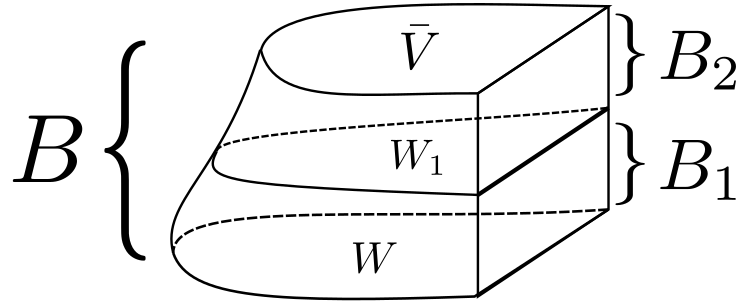
\includegraphics[width=50mm]{B1-B2}
		\end{figure}

		By construction, the bordism $B_{2}$ is the trace of surgeries of codimension
		$\geq 3$. Therefore, we can apply the equivariant version \cite[Theorem~2]{Hanke} of the Gromov--Lawson theorem to extend the
		metric $g_{\bar{V}}$ to a $G$-invariant metric of positive scalar curvature
		$g_{2}$ on $B_2$. Let us denote by $g_1$ the $G$ -invariant metric of positive
		scalar curvature obtained by restricting $g_{2}$ to~$W_{1}$.
		
The last fact to prove is that $\Psi_{|B_1}\colon B_1\to Y$ factors through $f\colon X\to Y$.
		Indeed, $B_1$ is obtained form $W$ by attaching, up to homotopy, cells
		of dimension up to~2. Define a~map $h\colon B_1\times \{0\}\cup W\times [0,1]\to Y$ as
		the restriction of $\Psi|_{B_1}\circ \mathrm{pr}$ to this subspace of $B_1\times [0,1]$, where~${\mathrm{pr}\colon
		B_1\times [0,1]\to B_1}$ is the obvious projection. Note that by assumption the
		restriction of this map to $W\times \{1\}$ equals $f\circ \varphi$. These are
		exactly the conditions of the relative precursor \cite[Proposition~2.5]{ttd}
		of Proposition~\ref{whitehead} which now implies in particular (because $f$ is
		$2$-connected) that there exists an extension $K\colon B_1\to X$ of
		$\varphi$.
		
		Now observe that $(B_1, \Phi, g_1)$ is a bordism between $(W,\varphi,g)$
		and the trivial cycle $(W_1,K|_{W_1},\allowbreak g_1|_{\partial W})$ in
		$R^{\rm spin}_n(X)^{G}$ (trivial because the metric extends to the metric $g_1$ of
		positive scalar curvature on all of $W_1$), the injectivity of $f_*$ is proved.
	\end{proof}
	
	
\begin{thebibliography}{99}
\bibitem[2]{Hanke}
Hanke B., Positive scalar curvature with symmetry,
 \href{https://doi.org/10.1515/CRELLE.2008.003}{\textit{J.~Reine Angew.
 Math.}} \textbf{614} (2008), 73--115,
 \href{http://arxiv.org/abs/math.GT/0512284}{arXiv:math.GT/0512284}.

\bibitem[3]{Mayer}
Mayer K.H., {$G$}-invariante {M}orse-{F}unktionen,
 \href{https://doi.org/10.1007/BF01173705}{\textit{Manuscripta Math.}}
 \textbf{63} (1989), 99--114.

\bibitem[4]{Milnor}
Milnor J., Lectures on the {$h$}-cobordism theorem, Princeton University Press,
 Princeton, NJ, 1965.

\bibitem[5]{PiazzaSchick}
Piazza P., Schick T., Rho-classes, index theory and {S}tolz' positive scalar
 curvature sequence,
 \href{https://doi.org/10.1112/jtopol/jtt048}{\textit{J.~Topol.}} \textbf{7}
 (2014), 965--1004, \href{http://arxiv.org/abs/1210.6892}{arXiv:1210.6892}.

\bibitem[10]{Stolz}
Stolz S., Concordance classes of positive scalar curvature metrics, {P}reprint, University of Notre Dame, 1999, \url{https://web.archive.org/web/20240430033820/https://www3.nd.edu/~stolz/concordance.ps}.

\bibitem[11]{tomDieck}
tom Dieck T., Orbittypen und \"aquivariante {H}omologie.~{I},
 \href{https://doi.org/10.1007/BF01304886}{\textit{Arch. Math. (Basel)}}
 \textbf{23} (1972), 307--317.

\bibitem[12]{ttd}
tom Dieck T., Transformation groups, \textit{De Gruyter Stud. Math.}, Vol.~8,
 \href{https://doi.org/10.1515/9783110858372.312}{Walter de Gruyter \& Co.},
 Berlin, 1987.

\bibitem[13]{Wasserman}
Wasserman A.G., Equivariant differential topology,
 \href{https://doi.org/10.1016/0040-9383(69)90005-6}{\textit{Topology}}
 \textbf{8} (1969), 127--150.

\bibitem[14]{XieYu}
Xie Z., Yu G., Positive scalar curvature, higher rho invariants and
 localization algebras,
 \href{https://doi.org/10.1016/j.aim.2014.06.001}{\textit{Adv. Math.}}
 \textbf{262} (2014), 823--866,
 \href{http://arxiv.org/abs/1302.4418}{arXiv:1302.4418}.

\bibitem[15]{XieYuZeidler}
Xie Z., Yu G., Zeidler R., On the range of the relative higher index and the
 higher rho-invariant for positive scalar curvature,
 \href{https://doi.org/10.1016/j.aim.2021.107897}{\textit{Adv. Math.}}
 \textbf{390} (2021), 107897, 24~pages,
 \href{http://arxiv.org/abs/1712.03722}{arXiv:1712.03722}.

\end{thebibliography}
\end{document}
